%%%%%%%%%%%%%%%%%%%%%%%%%%%%%%%%%%%%%%%%%%%%%%%%%%%%%%%%%%%%%%%%%%%%
%%%%%%%%%%%%%%%%%%%%%%%%%%%%%%%%%%%%%%%%%%%%%%%%%%%%%%%%%%%%%%%%%%%%
\section{Introdução} % Sections can be created in order to organize your presentation into discrete blocks, all sections and subsections are automatically printed in the table of contents as an overview of the talk


%\subsection{Referencial teórico} % A subsection can be created just before a set of slides with a common theme to further break down your presentation into chunks

\begin{frame}
\frametitle{Robótica}
\begin{columns}
	\column{0.35\linewidth}
	\begin{itemize}
	\item Industriais
	\item Médicos
	\item Móveis
		\begin{itemize}
		\item Com pernas (\textit{legged})
		\item Com rodas (\textit{wheeled})
		\end{itemize}
	\end{itemize}

	\column{0.7\linewidth}
	 \begin{figure}[h]
     \centering
     \captionsetup{width=\textwidth,font=footnotesize,textfont=bf}
     \begin{subfigure}[b]{0.5\textwidth}
 	\centering
         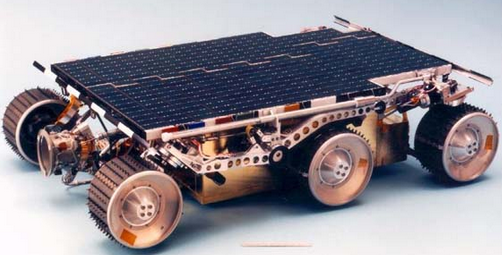
\includegraphics[width=\textwidth,height=\textheight,keepaspectratio]{Figuras/nasa.png}
         \caption{\centering \label{fig:Testen}}
     \end{subfigure}
     
     \begin{subfigure}[b]{0.5\textwidth}
 	\centering
         \includegraphics[width=\textwidth,height=5\textheight,keepaspectratio]{Figuras/Boston.png}
         \caption{\centering \label{fig:Testeo}}
     \end{subfigure}
	\caption{Robôs móveis: (a) Robô Sojourner (NASA,1997);(b) \textit{Legged Squad Support System} (DYNAMICS,2016)}
 \end{figure}
	
\end{columns}
\end{frame}

%------------------------------------------------

\begin{frame}
\frametitle{Controle de tempo contínuo}
\begin{columns}
	\column{0.45\linewidth}
	\begin{itemize}
	\item Malha aberta
	\item Malha fechada
	\item Controlador
		\begin{itemize}
		\item Proporcional
		\item Integral
		\item Derivativa
		\end{itemize}
	\end{itemize}
	
	\column{0.6\linewidth}
	\begin{figure}[h]
     \centering
     \captionsetup{width=\textwidth,font=footnotesize,textfont=bf}
     \begin{subfigure}[b]{\textwidth}
 	\centering
         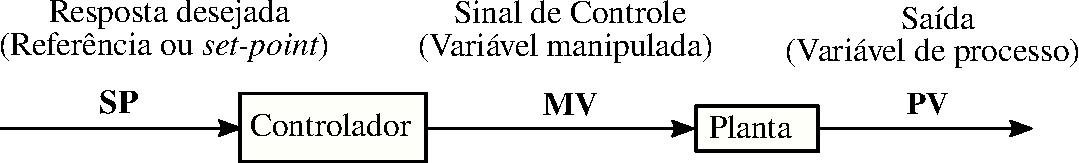
\includegraphics[width=\textwidth,height=\textheight,keepaspectratio]{Figuras/MalhaAberta.pdf}
         \caption{\centering \label{fig:jkl}}
     \end{subfigure}
     
     \begin{subfigure}[b]{\textwidth}
 	\centering
         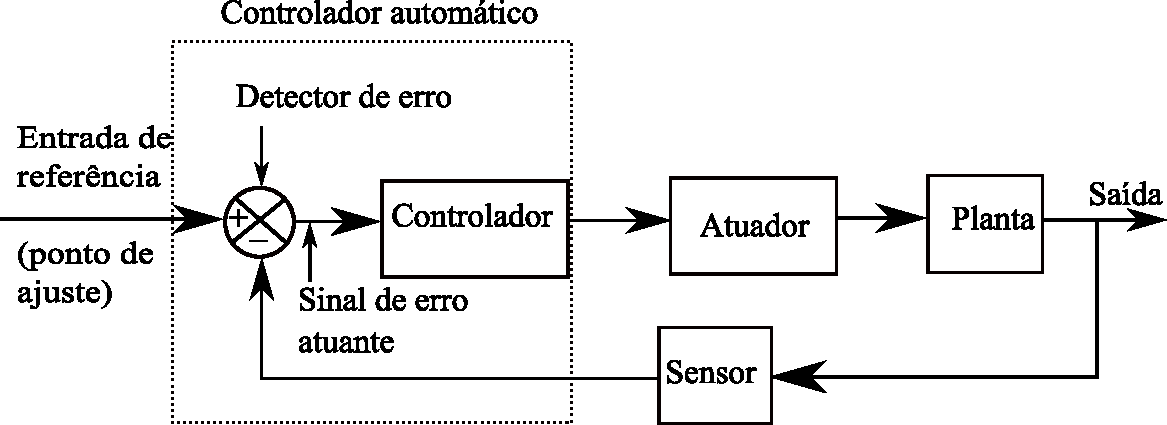
\includegraphics[width=\textwidth,height=5\textheight,keepaspectratio]{Figuras/Controlador.pdf}
         \caption{\centering \label{fig:ppolk}}
     \end{subfigure}
	\caption{Diagramas de controle: (a) Malha aberta;(b) Malha fechada com controlador}
 \end{figure}
	
\end{columns}
\end{frame}

%------------------------------------------------

\begin{frame}
\frametitle{Controle a eventos discretos}
\begin{columns}
	\column{0.3\linewidth}
	\begin{itemize}
	\item Eventos discretos
	\item Autômato
		\begin{itemize}
		\item Moore
		\item Mealy
		\end{itemize}
	\end{itemize}
	
	\column{0.7\linewidth}
	\begin{figure}[h]
     \centering
     \captionsetup{width=0.85\textwidth,font=footnotesize,textfont=bf}
     \begin{subfigure}[b]{\textwidth}
 	\centering
         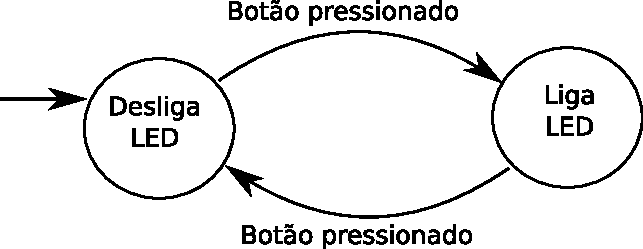
\includegraphics[width=0.85\textwidth,height=\textheight,keepaspectratio]{Figuras/moore.pdf}
         \caption{\centering \label{fig:moore}}
     \end{subfigure}
     
     \begin{subfigure}[b]{\textwidth}
 	\centering
         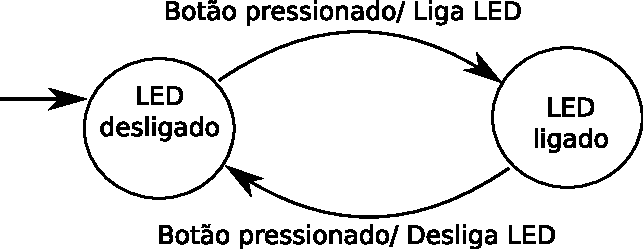
\includegraphics[width=0.85\textwidth,height=5\textheight,keepaspectratio]{Figuras/mealy.pdf}
         \caption{\centering \label{fig:mealy}}
     \end{subfigure}
	\caption{Autômatos: (a) Moore; (b) Mealy}
 \end{figure}
	
\end{columns}
\end{frame}


\begin{frame}
\frametitle{Trabalho de Petry (2016)}
\begin{columns}
	\column{0.3\linewidth}
	\begin{itemize}
	\item Controle híbrido
	\item Controlador PID
	\item Lógica \textit{fuzzy}
	\end{itemize}
	
	\column{0.7\linewidth}
	\begin{figure}[h]
     \centering
     \captionsetup{width=0.9\textwidth,font=footnotesize,textfont=bf}
     \begin{subfigure}[b]{0.4\textwidth}
 	\centering
         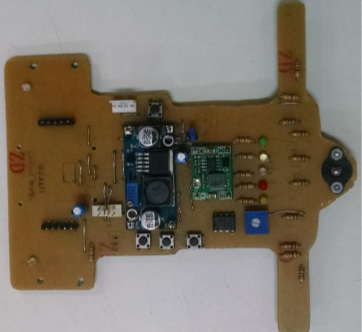
\includegraphics[width=1\textwidth,height=0.4\textheight]{Figuras/marcio1.png}
         \caption{\centering \label{fig:marcio1}}
     \end{subfigure}
	~     
     \begin{subfigure}[b]{0.4\textwidth}
 	\centering
         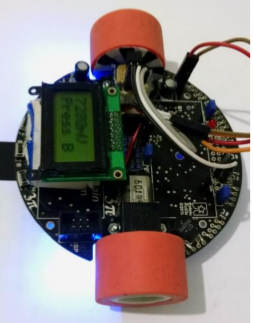
\includegraphics[width=1\textwidth,height=0.4\textheight]{Figuras/polulumod.png}
         \caption{\centering \label{fig:pololumarcio}}
     \end{subfigure}
	\caption{Robôs de Petry (2016): (a) \textit{Alpha project}; (b) Pololu 3pi modificado}
 \end{figure}
	
\end{columns}
\end{frame}

%------------------------------------------------

\section{Objetivos}

\begin{frame}
\frametitle{Objetivos}
\begin{block}{Geral}
	 Projetar e implementar um protótipo de um robô seguidor de linha, que seja autônomo, através da utilização de controle híbrido, aperfeiçoando as técnicas desenvolvidas por Petry (2016).
\end{block}

\begin{block}{Específicos}
	\begin{itemize}
	\item Projetar o condicionamento de sinais necessários para os dispositivos a serem utilizados, permitindo uma precisão na leitura dos sensores;
	\item Projetar e confeccionar a estrutura do protótipo, visando atender as dimensões especificadas pela Robocore;
	\item Implementar um controlador de Sistemas a Eventos Discretos, para que seja possível tratar de maneira precisa as marcações laterais da pista;

	\end{itemize}
\end{block}

\end{frame}

\begin{frame}
\frametitle{Objetivos}
\begin{block}{Específicos}
	\begin{itemize}
	\item Modelar a função de transferência do robô;
	\item Implementar um controlador para manter o robô sobre a linha na pista;
	\item Realizar testes com o protótipo em pistas que sigam as normas da Robocore;
	\item Fazer o mapeamento do percurso com um \textit{encoder para o controle da velocidade}
	\item Comparar os resultados obtidos com o de Petry (2016).
	\end{itemize}
\end{block}

\end{frame}

%------------------------------------------------

%\begin{frame}
%\frametitle{Multiple Columns}
%\begin{columns}[c] % The "c" option specifies centered vertical alignment while the "t" option is used for top vertical alignment
%
%\column{.45\textwidth} % Left column and width
%\textbf{Heading}
%\begin{enumerate}
%\item Statement
%\item Explanation
%\item Example
%\end{enumerate}
%
%\column{.5\textwidth} % Right column and width
%Lorem ipsum dolor sit amet, consectetur adipiscing elit. Integer lectus nisl, ultricies in feugiat rutrum, porttitor sit amet augue. Aliquam ut tortor mauris. Sed volutpat ante purus, quis accumsan dolor.
%
%\end{columns}
%\end{frame}

%------------------------------------------------
\section{Metodologia}

\begin{frame}
\frametitle{Metodologia}

	\begin{enumerate}
	\item Definição e aquisição dos componentes;
	\item Condicionamento de sinais dos sensores;
	\item Projeto da estrutura mecânica e \textit{software} embarcado;
	\item Projeto do controlador;
	\item Integração do sistema e implementação do protótipo;
	\item Testes de desempenho;
	\item Implementação do projeto final.
	\end{enumerate}
	
\end{frame}

%------------------------------------------------
\section{Justificativa}



\begin{frame}
\frametitle{Justificativa}
\begin{columns}[c]

	\column{0.4\textwidth}
	\begin{figure}[h]
     \centering
     \captionsetup{width=0.85\textwidth,font=footnotesize,textfont=bf}
     \begin{subfigure}[b]{\textwidth}
 	\centering
         
\includegraphics[width=0.85\textwidth,height=\textheight,keepaspectratio]{Figuras/robogames.jpg}
         \caption{\centering \label{fig:fss}}
     \end{subfigure}
     
     \begin{subfigure}[b]{\textwidth}
 	\centering
         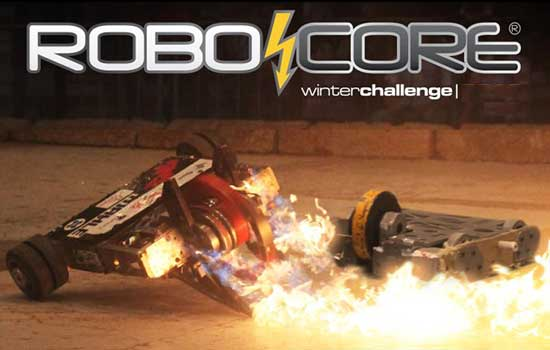
\includegraphics[width=0.85\textwidth,height=5\textheight,keepaspectratio]{Figuras/winterlogo.jpg}
         \caption{\centering \label{fig:vdd}}
     \end{subfigure}
	\caption{Autômatos: (a) Moore; (b) Mealy}
 \end{figure}
	\pause
	\column{0.6\textwidth}
	\begin{itemize}
	\item ART (\textit{ Autonomous Rail Rapid Transit} ou Trilho Autônomo de Trânsito 	Rápido)
	\item Trem em Zhuzhou (China)
	\end{itemize}

	\begin{figure}[]
	 \centering
	 \captionsetup{width=0.7\textwidth,font=footnotesize,textfont=bf}
	 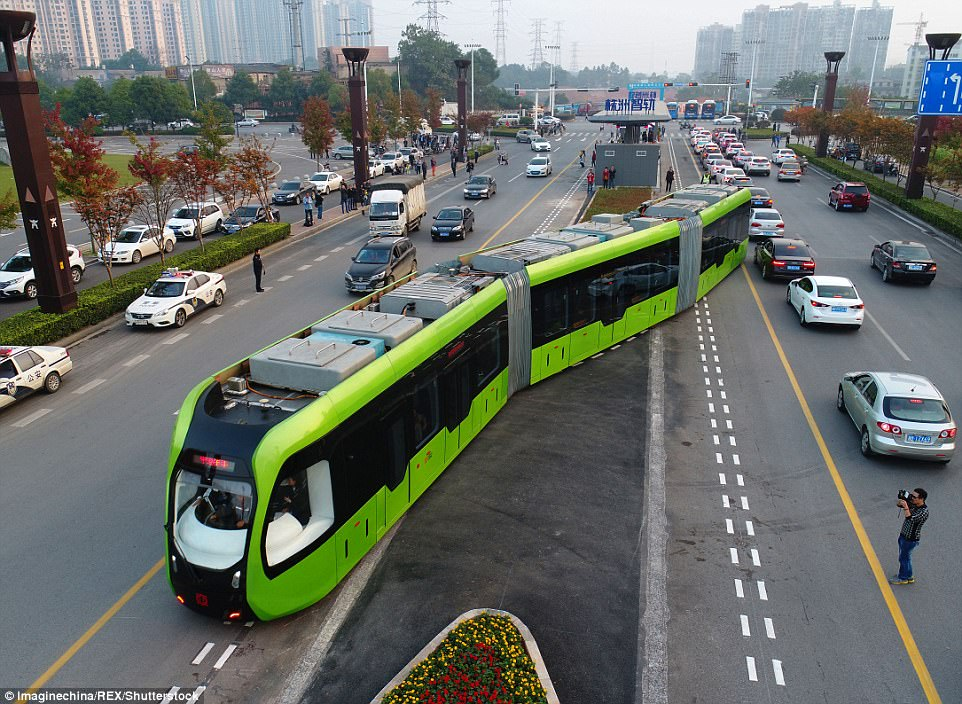
\includegraphics[width=0.7\textwidth,keepaspectratio]{Figuras/Trem.jpg}
	 \caption{Trem sobre trilhos virtuais (DAILYMAIL, 2017)}
	\end{figure}

\end{columns}
\end{frame}


%%%%%%%%%%%%%%%%%%%%%%% EOF %%%%%%%%%%%%%%%%%%%%%%%%%%%%